\documentclass[a4paper]{report}
\usepackage[
  a4paper,
  margin=1.5cm,
  top=70pt,
  headheight=30pt,
]{geometry}  




% \usepackage[spanish]{babel}
\usepackage{amssymb}
\usepackage{amsfonts}
\usepackage{amsmath}
\usepackage{amsmath,eqparbox}
\usepackage{array}
\usepackage{bm}
\usepackage{blindtext}
\usepackage{caption}
\usepackage[makeroom]{cancel}
\usepackage{euscript}[mathcal]
\usepackage{enumitem}
\usepackage{fontenc}
\usepackage{gensymb}
\usepackage{graphicx}
\usepackage{lastpage}
\usepackage{multirow}
\usepackage{setspace}
\usepackage{titlesec}
\usepackage{xcolor}
\usepackage{float}
\usepackage{verbatim}
\usepackage{comment}
\excludecomment{debug}
\usepackage{subcaption}

%% Renew commands
\renewcommand{\figurename}{Fig.}
\captionsetup{font=footnotesize}

%%  ----- Cabecera y pie de pagina -----
\usepackage{fancyhdr}
\pagestyle{fancy}
\fancyhead{}
\fancyhead[L]{UNCuyo - Ing. Mecatrónica \\ Mendoza - Argentina - 2025 \\ \hspace{0.1pt}}
\fancyhead[C]{317 - Automátas y Control Discreto \\ \hspace{0.5pt} \\ \textbf{Proyecto Final de Estudios: Robot cosechador automático}}
\fancyhead[R]{Brenda Gudiño \\ Alan Vignolo \\ \hspace{0.5pt}}

\fancyfoot{}
\fancyfoot[R]{Página \thepage \hspace{2pt} de \pageref{LastPage}} 

%% Para ver cabecera y pie de pagina en los inicios de capitulo
\fancypagestyle{plain}{
\fancyhead{}
\fancyhead[L]{UNCuyo - Ing. Mecatrónica \\ Mendoza - Argentina - 2024 \\ \hspace{0.1pt}}
\fancyhead[C]{Proyecto final de estudios \\ \hspace{0.5pt} \\ \textbf{Robot cosechador automático}}
\fancyhead[R]{Brenda Gudiño \\ Alan Vignolo  \\ \hspace{0.5pt}}

\fancyfoot{}
\fancyfoot[R]{Página \thepage \hspace{2pt} de \pageref{LastPage}} 
}

%% -------------------------------------
%% Indice y capitulos ----------------------------
\renewcommand*\contentsname{Índice}
\titleformat{\chapter}[block]
  {\normalfont\huge\bfseries}{\thechapter.}{1em}{\Huge}
\titlespacing*{\chapter}{0pt}{0pt}{10pt}
%% ------------------------------------




%% Portada ------------------------------
\title{

\includegraphics[scale = 0.3]{logo_uncuyo.png} \\ [2cm]
{\Huge \textbf{Proyecto final de estudios} \\ [1cm] 
Cosechador de Lechugas Autónomo con Unidad de Detección por Inteligencia Optica}}
\author{Brenda Gudiño \\ Alan Vignolo}

\date{Fecha de presentación \\ XX/XX/2025}
%% -------------------------------------
\begin{document}


\maketitle
\tableofcontents


%% RESUMEN \\\\\\\\\\\\\\\\\\\\\\\\\\\\
\newpage
\chapter{Resumen}
En el presente informe se detalla el desarrollo del proyecto final de estudios de Ingeniería Mecatrónica, el mismo consiste en un robot cosechador automático de lechugas hidropónicas con posicionamiento ajustador por inteligencia artificial. En el transcurso del informe se desarrollan el modelado mecánico y electrónico de la estructura, montaje, control, pruebas, resultados finales y posibles mejoras.
%% INTRODUCCION \\\\\\\\\\\\\\\\\\\\\\\\\\\\
\newpage
\chapter{Introducción}
El presente informe expone el desarrollo de un robot cosechador automático de lechugas, cuyo objetivo principal es optimizar las labores de recolección en entornos de cultivo, mejorando la eficiencia del proceso y reduciendo la necesidad de intervención manual. Para lograrlo, se abordaron diferentes etapas de diseño, modelado, montaje, control e implementación de interfaces, las cuales se estructuran en este documento siguiendo la lógica de construcción del sistema.

En la sección 3 se detallan los aspectos técnicos y metodológicos empleados. Se inicia con el modelado (3.1), que comprende el diseño mecánico del sistema, la elaboración de modelos CAD y su posterior impresión 3D, así como la descripción de la estructura que soporta los diferentes subsistemas. A continuación, en el apartado de electrónica y componentes, se enumeran y justifican los elementos electrónicos seleccionados, desde sensores hasta actuadores, que permiten al robot cumplir con sus funciones.

Posteriormente, se presenta el montaje, donde se integran tanto las partes mecánicas como electrónicas, conformando el prototipo físico del robot. La subsección de control aborda dos dimensiones fundamentales: el control de movimiento, que asegura la correcta navegación y operación del sistema, y la creación y uso de inteligencia artificial, la cual dota al robot de capacidades de reconocimiento y toma de decisiones frente a las condiciones de cultivo. Finalmente, se incluye el desarrollo de la interfaz, pensada para la interacción entre el usuario y el sistema, garantizando facilidad de uso y monitoreo eficiente.

Por último, se documentan los ensayos realizados sobre el prototipo, evaluando su desempeño en el ciclo normal de trabajo y en otras situaciones.
%% DESARROLLO \\\\\\\\\\\\\\\\\\\\\\\\\\\\
\chapter{Desarrollo}
\section{Modelado}
\subsection{Modelado del sistema mecánico}
\input{Modelado/Modelado_mecánico}
\subsection{Modelado CAD e impresión 3D}
\subsection{Modelado CAD para prototipo}
En esta sección se muestran los diseños implementados y utilizados en el prototipo, a diferencia de los diseños propuestos antes, estos cuentan con canales para el pasaje de los cables y con detalles que surgieron de las distintas impresiones y pruebas previas que guiaron hacia el resultado y diseño final de cada soporte para la implementación en el prototipo.
\subsubsection{Suporte superior}
El soporte superior (fig. \ref{fig:Superior_orginal}) es el que recibe la mayor carga en la estructura, ya que debe soportar el peso de la estructura vertical (soportes, brazo robótico, varillas). Para ello se debe realizar un analisis de carga y deformación previos para verificar si la forma del soporte es la adecuada para tolerar los esfuerzos.
\begin{figure}[H]
    \centering
    \begin{subfigure}[b]{0.35\textwidth}
        \centering
        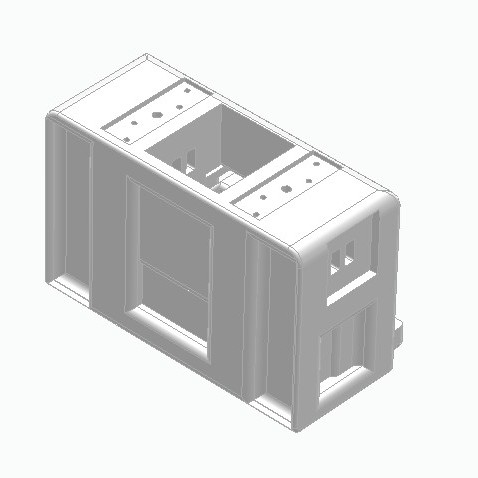
\includegraphics[width=0.75\textwidth]{img/Superior_frente.jpg}
        \caption{Frente del soporte superior.}
        \label{fig:izaje_desacoplado}
    \end{subfigure}
    \hspace{0.02\textwidth}
    \begin{subfigure}[b]{0.35\textwidth}
        \centering
        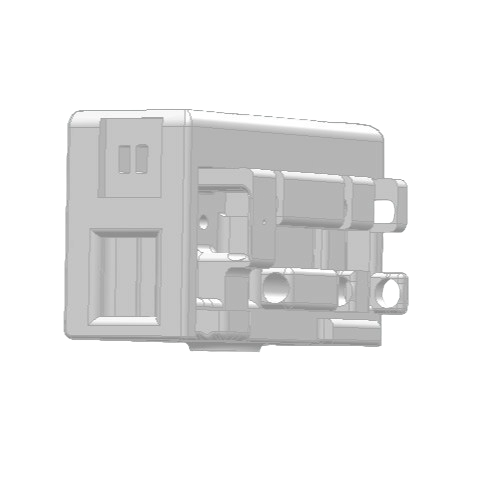
\includegraphics[width=0.75\textwidth]{img/superior_atras.jpg}
        \caption{Posterior del soporte superior.}
        \label{fig:izaje_acoplado}
    \end{subfigure}
     \caption{Soporte superior.}
    \label{fig:Superior_orginal}
\end{figure}
Para realizar el análisis de esfuerzos y deformación se simplificó la pieza ya que el solver del software utilizado no podía procesar y analizar geometrías tan complejas como la planteada. Además se tomaron las propiedades del filamento plástico PETG de impresión 3D para hacer un correcto analisis.\\
En la siguiente figura se pueden observar las fuerzas aplicadas, las mismas contemplan una carga máxima de 3.5kg. Las fuerzas son aplicadas en las secciones indicadas en la imagen y dividas en dos para la parte superior y en tres para la parte inferior.\\
\begin{figure}[H]
    \centering
        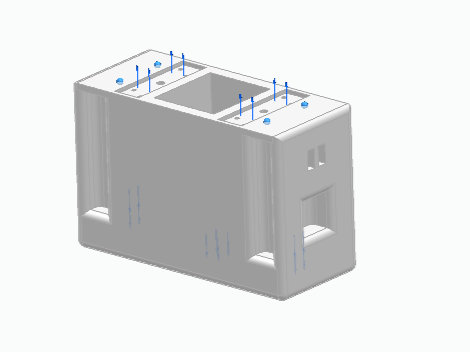
\includegraphics[width=0.5\textwidth]{img/Fuerzas_superiores.png} \par
        \caption{\textit{Fuerzas aplicadas para el análisis}}
        \label{fig:fuerzas_sup}
\end{figure}
%    
%\end{figure} 
Como se puede observar en las imágenes, la tensión está muy por debajo de la tensión de rotura y las deformaciones son prácticamente insignificantes, por lo que se puede concluir que el diseño es aplicable.\\
\begin{figure}[H]
    \centering
    \begin{subfigure}{0.35\textwidth}
        \centering
        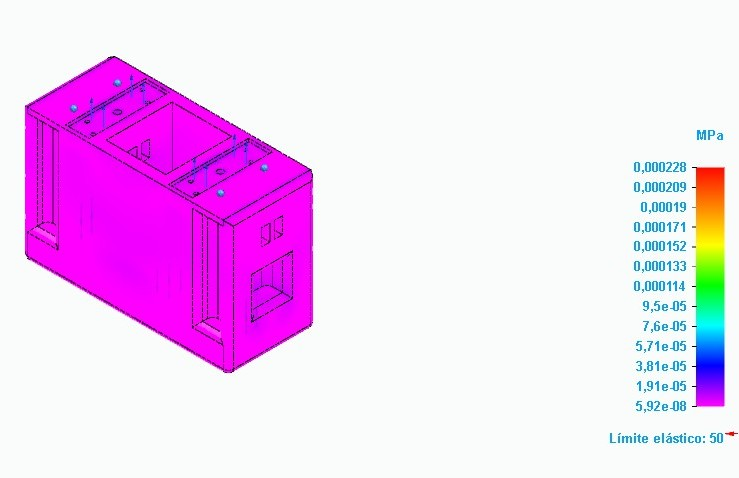
\includegraphics[width=0.8\textwidth]{img/completo_sin_mallar.jpg} \par
        \caption{\textit{Análisis de tensión de Von Misses.}}
        \label{fig:sup_analisis_tension}
    \end{subfigure}
    \hspace{0.5cm}
    \begin{subfigure}{0.35\textwidth}
        \centering
        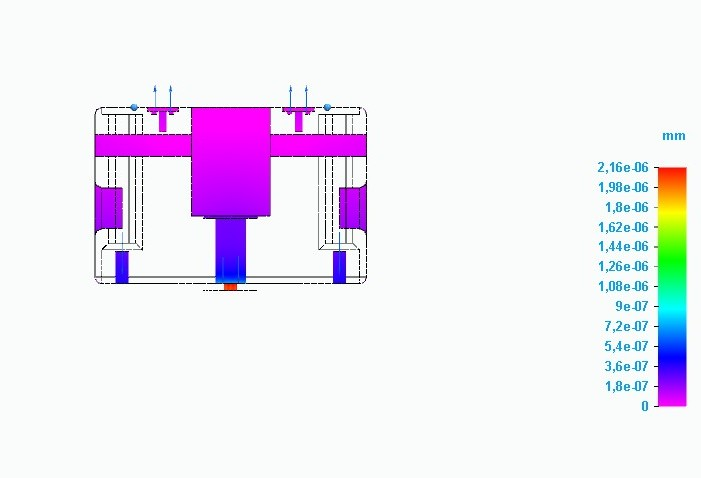
\includegraphics[width=0.8\textwidth]{img/Corte_transv_sin_mallado_def.jpg} \par
        \caption{\textit{Análisis de deformación.}}
        \label{fig:sup_analisis_def}
    \end{subfigure}
    \caption{Soporte superior. Resultados de analisis de esfuerzos y deformaciones.}
\end{figure}

\subsubsection{Suporte medio}
Este soporte se desplaza por el movimiento de la varilla, además es en donde se encuentra el brazo robótico y la cámara. Cuenta con canales internos para el montaje de los cables. \\
\begin{figure}[H]
    \centering
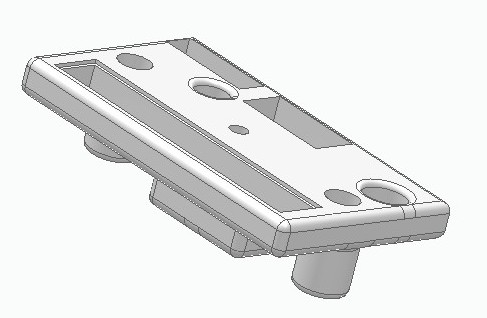
\includegraphics[width=0.45\textwidth]{img/medio.jpg} \par
    \caption{\textit{Soporte medio.}}
    \label{fig:soporte_medio}
\end{figure}

\subsubsection{Suporte inferior}
Este soporte cierra la estructura vertical, en el van los extremos de las varillas trefiladas y la varilla roscada y el final de carrera correspondiente. También cuenta con canales internos para el montaje de los cables. \\
\begin{figure}[H]
    \centering
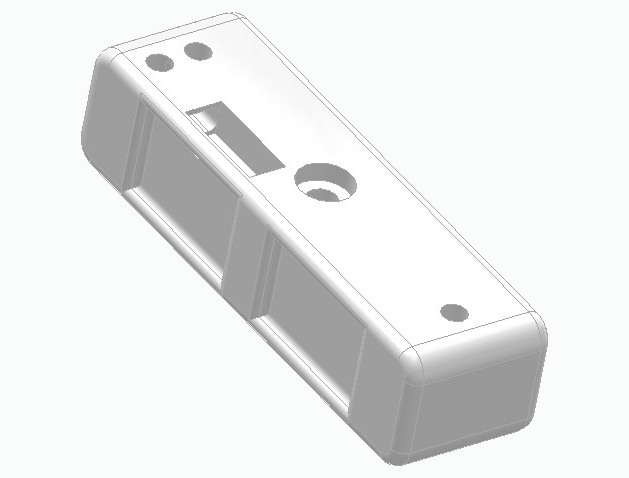
\includegraphics[width=0.45\textwidth]{img/inferior_completo.jpg} \par
    \caption{\textit{Soporte inferior.}}
    \label{fig:soporte_inferior}
\end{figure}

\subsubsection{Robot serie}
Para el diseño del brazo robótico se tienen 2 partes principales, el cuerpo del brazo y el efector final o gripper. \\
El diseño del gripper tiene en cuenta un sistema de transmisión piñon-cremallera para el agarre, igual que el de la  fig. \ref{fig:gripper_Real_transmision}. La diferencia entre ambos robots serie no radica en el diseño si no en el material. Este brazo se plantea para ser impreso en PETG/PLA.\\

\begin{figure}[H]
    \centering
    \begin{subfigure}{0.35\textwidth}
        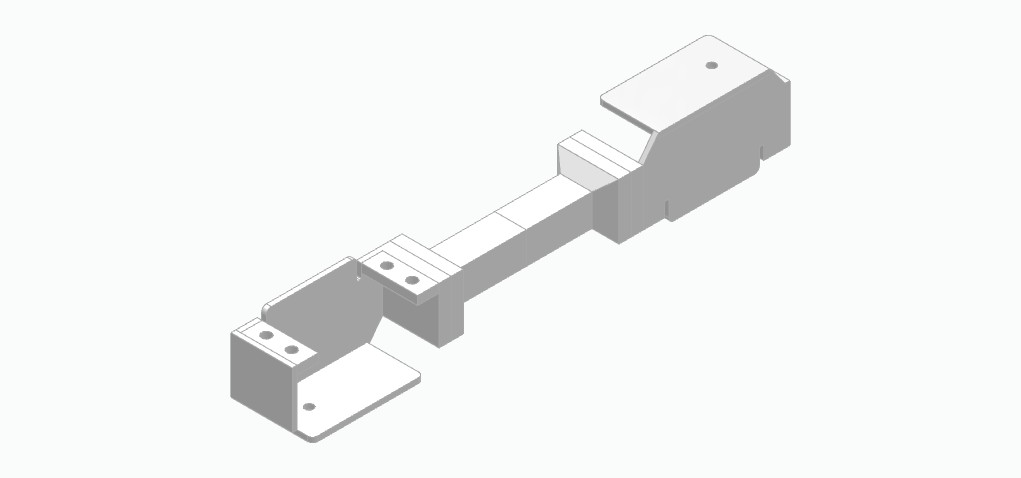
\includegraphics[width=\textwidth]{img/brazo_medio.jpg} \par
    \caption{\textit{Cuerpo del brazo.}}
    \label{fig:brazo}
    \end{subfigure}
    \hspace{0.5cm}
    \begin{subfigure}{0.35\textwidth}
        \centering
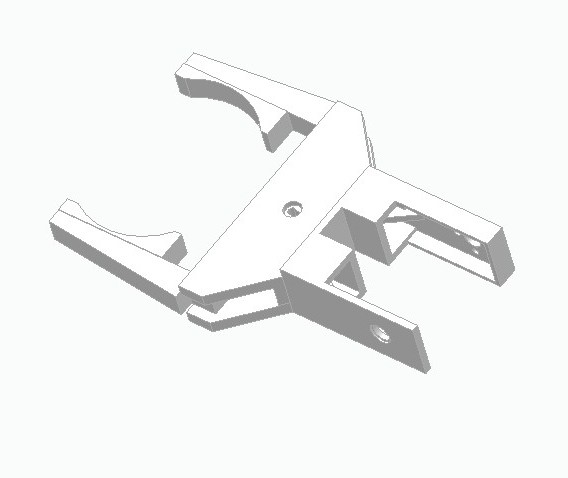
\includegraphics[width=\textwidth]{img/pinza.jpg} \par
    \caption{\textit{Gripper.}}
    \label{fig:gripper}
    \end{subfigure}
    \caption{Piezas principales del robot serie.}
\end{figure}
\subsection{Estructura}
Para la implementación de este proyecto se propone una estructura con movimientos semejantes a los de una estructura cartesiana, la misma se pensó para amurar a la pared pero por cuestiones de espacio disponible se tuvo que diseñar una estructura con caños estructurales móvil para poder hacer el montaje de los sistemas mecánicos.\\
Por otro lado, como lo que se quiere mostrar principalmente es el movimiento y control de la estructura, el sistema hidropónico se simplificó en dos tubos de pvc horizontales y paralelos montados sobre la pared de la estructura que fue hecha a partir de tablas de madera.\\
\textbf{Poner foto de la estructura}
\section{Electrónica y componentes}
\input{{Control}/Electronica_componentes}
\section{Montaje}
\section{Control}
\subsection{Control de movimiento}
\subsection{Inteligencia Artificial y Sistemas de Visión}
\subsection{Creación y Uso de Inteligencia Artificial}

El desarrollo del robot cosechador incorpora una arquitectura integral de inteligencia artificial diseñada para abordar los desafíos específicos de la agricultura automatizada. La implementación combina técnicas de visión por computadora, aprendizaje profundo y algoritmos de procesamiento de imágenes especializados, conformando un sistema autónomo capaz de percibir, analizar y responder a las condiciones variables del entorno de cultivo hidropónico.

\begin{figure}[h]
\centering
\includegraphics[width=0.8\textwidth]{imagenes/arquitectura_ia_general.png}
\caption{Arquitectura integral de inteligencia artificial del robot cosechador mostrando la interconexión de módulos especializados}
\label{fig:arquitectura_ia_general}
\end{figure}

La arquitectura de IA se fundamenta en la integración de múltiples módulos especializados que operan de manera coordinada. Esta aproximación modular permite optimizar cada componente para tareas específicas mientras mantiene la flexibilidad necesaria para adaptarse a diferentes escenarios operativos. El sistema procesa información visual en tiempo real, ejecuta algoritmos de toma de decisiones y proporciona retroalimentación continua para el control preciso de los actuadores mecánicos.

La selección de las tecnologías empleadas se basó en criterios de robustez, rapidez,eficiencia computacional y precisión operativa. Se implementaron algoritmos de procesamiento de imágenes utilizando OpenCV para las tareas de detección y segmentación, mientras que TensorFlow y Keras proporcionan el framework para los modelos de aprendizaje profundo. Esta combinación tecnológica permite al sistema operar en condiciones variables de iluminación y enfrentar la diversidad morfológica natural de los cultivos.

\begin{figure}[h]
\centering
\includegraphics[width=0.9\textwidth]{imagenes/pipeline_procesamiento_imagenes.png}
\caption{Flujo completo del pipeline de procesamiento de imágenes desde captura hasta extracción de características}
\label{fig:pipeline_procesamiento}
\end{figure}

El procesamiento de imágenes constituye el núcleo de la percepción artificial del robot. Las imágenes capturadas por el sistema de cámaras se someten a una secuencia de transformaciones que incluyen conversiones de espacios de color, filtrado de ruido, segmentación por umbralización y análisis morfológico. Estos procesos permiten extraer características relevantes del entorno, identificar elementos de interés y calcular parámetros geométricos necesarios para la navegación y manipulación precisas.

La implementación de redes neuronales convolucionales permite al robot desarrollar capacidades de reconocimiento visual sofisticadas. Los modelos entrenados procesan las características extraídas de las imágenes para clasificar estados de cultivo, evaluar la madurez de las plantas y determinar estrategias de cosecha apropiadas. La arquitectura de red implementada utiliza capas convolucionales para la extracción de características, seguidas de capas densas para la clasificación final.

\subsubsection{Sistema de Posicionamiento Inteligente}

El sistema de posicionamiento inteligente constituye la base de la navegación precisa del robot, implementando algoritmos de visión artificial que permiten el alineamiento exacto frente a cada espacio de cultivo. Este módulo utiliza elementos de referencia visual estratégicamente ubicados para calcular correcciones de posición en tiempo real, garantizando la precisión necesaria para las operaciones de cosecha.

La metodología de detección emplea cintas negras adheridas sobre los tubos de PVC como elementos de contraste visual. Estos marcadores proporcionan puntos de referencia detectables que facilitan el cálculo de correcciones de posición en los ejes X e Y. El algoritmo desarrollado maximiza la robustez frente a variaciones ambientales mediante técnicas de procesamiento adaptativo.

El proceso de detección implementa una secuencia optimizada que inicia con la captura de imágenes RGB del entorno objetivo. La imagen adquirida se convierte al espacio de color HSV, extrayendo el canal V (brillo) para eliminar variaciones cromáticas y enfocar el análisis en el contraste de luminosidad. Esta transformación resulta fundamental para mantener la consistencia de detección bajo diferentes condiciones de iluminación.

\begin{figure}[h]
\centering
\includegraphics[width=0.7\textwidth]{imagenes/transformacion_rgb_hsv.png}
\caption{Comparación visual entre espacios de color RGB y HSV para optimización de detección}
\label{fig:transformacion_rgb_hsv}
\end{figure}

La transformación al espacio HSV se define matemáticamente como:

\begin{equation}
I_{HSV} = \text{cvtColor}(I_{RGB}, \text{COLOR\_RGB2HSV})
\end{equation}

\begin{equation}
I_V = I_{HSV}[:,:,2]
\end{equation}

donde $I_V$ representa el canal de valor (brillo) que resulta invariante a los cambios de tonalidad e intensidad cromática.

Posteriormente se aplica una umbralización binaria inversa con valor de referencia de 50 para destacar las regiones oscuras correspondientes a las cintas negras. Este valor de referencia se determinó mediante análisis empírico del histograma de intensidades, identificando el punto óptimo de separación entre el fondo y los elementos de referencia. La umbralización inversa (THRESH\_BINARY\_INV) produce píxeles blancos en las zonas de interés, facilitando la posterior detección de contornos:

\begin{figure}[h]
\centering
\includegraphics[width=0.6\textwidth]{imagenes/umbralizacion_binaria.png}
\caption{Proceso de umbralización binaria inversa con umbral T=50 para detección de cintas de referencia}
\label{fig:umbralizacion_binaria}
\end{figure}

\begin{equation}
I_{binary}(x,y) = \begin{cases} 
255 & \text{si } I_V(x,y) < T \\
0 & \text{si } I_V(x,y) \geq T
\end{cases}
\end{equation}

donde $T = 50$ representa el umbral de binarización seleccionado empíricamente mediante maximización del contraste entre señal y ruido.

El algoritmo identifica contornos en la imagen binaria mediante el método de detección de contornos de OpenCV (algoritmo de Suzuki-Abe), aplicando filtros de área mínima de 500 píxeles para eliminar elementos espurios. Se implementa una evaluación de calidad que analiza el 10\% inferior del bounding box de cada contorno, permitiendo distinguir entre elementos de referencia válidos y ruido visual. Esta estrategia elimina la detección errónea de plantas y/o vasos en la imagen, asegurando que la referencia corresponda únicamente al borde inferior de la cinta.

\begin{figure}[h]
\centering
\includegraphics[width=0.8\textwidth]{imagenes/deteccion_contornos.png}
\caption{Visualización de contornos identificados superpuestos sobre imagen original con filtrado de área}
\label{fig:deteccion_contornos}
\end{figure}

La evaluación de calidad de base se define como:

\begin{equation}
Q_{base} = \frac{1}{A_{base}} \sum_{(x,y) \in R_{base}} I_{binary}(x,y)
\end{equation}

donde $R_{base}$ representa la región correspondiente al 10\% inferior del bounding box y $A_{base}$ es el área de dicha región.

La selección del mejor candidato se realiza mediante un algoritmo de scoring multicriteria que evalúa:

\begin{itemize}
    \item \textbf{Área del contorno}: Priorizando elementos con dimensiones apropiadas.
    \item \textbf{Posición relativa al centro}: Favoreciendo elementos cercanos al centro de la imagen.
    \item \textbf{Calidad de base}: Analizando la consistencia de la región inferior del contorno.
    \item \textbf{Factibilidad geométrica}: Verificando proporciones y orientación.
\end{itemize}

\begin{figure}[h]
\centering
\includegraphics[width=0.7\textwidth]{imagenes/scoring_multicriteria.png}
\caption{Representación gráfica del algoritmo de scoring multicriteria para selección del mejor candidato}
\label{fig:scoring_multicriteria}
\end{figure}

La función de scoring se expresa matemáticamente como:

\begin{equation}
\text{Score} = w_1 \cdot A_{norm} + w_2 \cdot P_{cent} + w_3 \cdot Q_{base}
\end{equation}

donde los pesos de ponderación se determinaron experimentalmente como $w_1 = 0.3$, $w_2 = 0.4$, $w_3 = 0.3$, optimizando la precisión de detección mediante validación cruzada. Los términos individuales se definen como:

\begin{equation}
A_{norm} = \frac{A_{contorno} - A_{min}}{A_{max} - A_{min}}
\end{equation}

\begin{equation}
P_{cent} = 1 - \frac{\sqrt{(C_x - I_{center_x})^2 + (C_y - I_{center_y})^2}}{D_{max}}
\end{equation}

donde $A_{contorno}$ es el área del contorno candidato, $A_{min}$ y $A_{max}$ son los límites de área válidos, $C_{x,y}$ son las coordenadas del centroide y $D_{max}$ es la máxima distancia euclidiana posible desde el centro.

El cálculo de corrección determina la distancia en píxeles entre el centro de la imagen y el centroide del elemento de referencia seleccionado. Esta información se convierte a unidades métricas mediante calibración lineal obtenida experimentalmente, proporcionando comandos de movimiento precisos para los actuadores.

La calibración pixel-métrica se realizó mediante regresión lineal por mínimos cuadrados, obteniendo las siguientes relaciones:

\textbf{Calibración Horizontal:}
\begin{equation}
\text{Corrección}_x = (C_x - I_{center\_x}) \cdot K_{cal\_x} + b_x
\end{equation}

donde $K_{cal\_x} = 0.3877$ mm/píxel y $b_x = 0.15$ mm, con coeficiente de determinación $R^2 = 0.9996$ y error promedio de $0.52$ mm.

\textbf{Calibración Vertical:}
\begin{equation}
\text{Corrección}_y = (C_y - I_{center\_y}) \cdot K_{cal\_y} + b_y
\end{equation}

Los parámetros de calibración se determinaron mediante un proceso de medición sistemática que incluyó 44 puntos de referencia distribuidos uniformemente en el rango operativo del sistema. La función de calibración lineal se expresa como:

\begin{equation}
\mathbf{K} = (\mathbf{X}^T\mathbf{X})^{-1}\mathbf{X}^T\mathbf{y}
\end{equation}

donde $\mathbf{X}$ es la matriz de observaciones en píxeles, $\mathbf{y}$ es el vector de mediciones reales en milímetros, y $\mathbf{K}$ contiene los coeficientes de calibración.

La precisión del sistema de posicionamiento se validó mediante análisis estadístico de 100 mediciones independientes, obteniendo una desviación estándar de $\sigma = 0.8$ mm y un error máximo absoluto de $1.35$ mm, cumpliendo con los requerimientos de precisión establecidos para las operaciones de cosecha.

El algoritmo implementa corrección iterativa con criterio de convergencia basado en tolerancia absoluta:

\begin{equation}
|\text{Corrección}_{i+1}| < \epsilon
\end{equation}

donde $\epsilon = 1.0$ mm representa la tolerancia de posicionamiento requerida para garantizar el éxito de las operaciones de manipulación.

\begin{figure}[h]
\centering
\includegraphics[width=0.6\textwidth]{imagenes/correccion_posicion_horizontal.png}
\caption{Resultado del algoritmo de corrección horizontal con cálculo de desviación en píxeles}
\label{fig:correccion_horizontal}
\end{figure}

\begin{figure}[h]
\centering
\includegraphics[width=0.6\textwidth]{imagenes/correccion_posicion_vertical.png}
\caption{Resultado del algoritmo de corrección vertical con evaluación de calidad de base}
\label{fig:correccion_vertical}
\end{figure}

\subsubsection{Sistema de Detección y Clasificación de Lechugas}

El módulo de detección y clasificación implementa una red neuronal convolucional especializada para el reconocimiento de lechugas en diferentes estados de desarrollo. El sistema combina técnicas de visión por computadora clásica para la detección de regiones de interés con aprendizaje profundo para la clasificación precisa del estado de madurez.

\begin{figure}[h]
\centering
\includegraphics[width=0.9\textwidth]{imagenes/arquitectura_cnn.png}
\caption{Arquitectura de la red neuronal convolucional implementada para clasificación de lechugas}
\label{fig:arquitectura_cnn}
\end{figure}

La arquitectura de red neuronal implementada utiliza una configuración modificada basada en principios de redes convolucionales profundas. La red procesa imágenes de entrada de 224×224 píxeles, dimensión seleccionada para optimizar el balance entre precisión de detección y eficiencia computacional en el hardware disponible.

\begin{equation}
\mathbf{X}_{input} \in \mathbb{R}^{224 \times 224 \times 3}
\end{equation}

La red se estructura en múltiples capas convolucionales que extraen características jerárquicas de las imágenes de entrada:

\begin{equation}
\mathbf{F}^{(l+1)} = \sigma(\mathbf{W}^{(l)} * \mathbf{F}^{(l)} + \mathbf{b}^{(l)})
\end{equation}

donde $\mathbf{F}^{(l)}$ representa el mapa de características de la capa $l$, $\mathbf{W}^{(l)}$ son los filtros convolucionales, $*$ denota la operación de convolución y $\sigma$ es la función de activación ReLU.

El preprocesamiento de imágenes implementa normalización automática y técnicas de aumento de datos para mejorar la robustez del modelo. Las imágenes se normalizan al rango [0,1] y se aplican transformaciones aleatorias durante el entrenamiento:

\begin{equation}
\mathbf{X}_{normalized} = \frac{\mathbf{X}_{input}}{255.0}
\end{equation}

\begin{figure}[h]
\centering
\includegraphics[width=0.8\textwidth]{imagenes/deteccion_caracteristicas_morfologicas.png}
\caption{Análisis de características morfológicas de lechugas mediante procesamiento de contornos}
\label{fig:caracteristicas_morfologicas}
\end{figure}

El sistema de detección complementa la clasificación neuronal con análisis de contornos para identificar regiones de interés dentro de las imágenes. Este enfoque híbrido permite localizar plantas individuales y evaluar características morfológicas relevantes para la toma de decisiones de cosecha.

La función de pérdida implementada utiliza entropía cruzada categórica para el entrenamiento multiclase:

\begin{equation}
\mathcal{L} = -\frac{1}{N} \sum_{i=1}^{N} \sum_{j=1}^{C} y_{ij} \log(\hat{y}_{ij})
\end{equation}

donde $N$ es el número de muestras, $C$ es el número de clases, $y_{ij}$ es la etiqueta verdadera y $\hat{y}_{ij}$ es la predicción del modelo.

\begin{figure}[h]
\centering
\includegraphics[width=0.8\textwidth]{imagenes/metricas_entrenamiento.png}
\caption{Evolución de loss y accuracy durante el proceso de entrenamiento de la red neuronal}
\label{fig:metricas_entrenamiento}
\end{figure}

\begin{figure}[h]
\centering
\includegraphics[width=0.6\textwidth]{imagenes/matriz_confusion.png}
\caption{Matriz de confusión mostrando resultados de clasificación del modelo entrenado}
\label{fig:matriz_confusion}
\end{figure}

\subsubsection{Mapeo Inteligente del Entorno de Cultivo}

El sistema de mapeo inteligente permite al robot construir una representación completa del entorno de cultivo hidropónico mediante exploración autónoma. El proceso opera en fases secuenciales que aprovechan la geometría estructurada del sistema para maximizar la eficiencia de exploración, implementando algoritmos de procesamiento en tiempo real sincronizados con el movimiento mecánico del robot.

La arquitectura del sistema de mapeo integra múltiples componentes que operan de manera coordinada: el controlador de movimiento, el sistema de visión artificial, el procesador de imágenes en tiempo real y el gestor de datos espaciales. Esta integración permite realizar detección continua mientras el robot se desplaza, optimizando el tiempo total de exploración.

El sistema implementa procesamiento de imágenes en tiempo real utilizando una arquitectura de streaming de video optimizada para operar a 10 FPS durante las fases de exploración. Esta frecuencia se seleccionó para balancear la precisión de detección con la eficiencia computacional, considerando la velocidad de movimiento del robot durante el mapeo.

La sincronización entre captura de imágenes y posición del robot se logra mediante un sistema de timestamps coordinado:

\begin{equation}
t_{captura}(i) = t_{inicio} + i \cdot \Delta t_{frame}
\end{equation}

donde $\Delta t_{frame} = 100$ ms corresponde al período entre frames a 10 FPS.

La posición instantánea del robot se calcula mediante interpolación lineal entre las posiciones reportadas por el sistema de control:

\begin{equation}
\mathbf{P}(t) = \mathbf{P}_{n-1} + \frac{t - t_{n-1}}{t_n - t_{n-1}}(\mathbf{P}_n - \mathbf{P}_{n-1})
\end{equation}

donde $\mathbf{P}(t) = [x(t), y(t)]^T$ representa la posición interpolada en el instante $t$.

\textbf{Algoritmo de Detección Temporal con Cooldown}

Para evitar detecciones múltiples del mismo elemento durante el movimiento continuo, se implementa un algoritmo de cooldown espacial que establece una distancia mínima de 50 mm entre detecciones consecutivas:

\begin{equation}
\text{Detección válida} = \begin{cases}
\text{True} & \text{si } ||\mathbf{P}_{actual} - \mathbf{P}_{última}||_2 \geq d_{cooldown} \\
\text{False} & \text{en caso contrario}
\end{cases}
\end{equation}

donde $d_{cooldown} = 50$ mm y $||\cdot||_2$ representa la norma euclidiana.

\textbf{Fase 1: Escaneo Vertical para Detección de Tubos}

La primera fase ejecuta un escaneo vertical desde la posición de referencia (0,0), durante el cual el robot se desplaza con velocidad reducida de 8000 pasos/segundo (equivalente a 40 mm/s considerando la relación de conversión $K_v = 200$ pasos/mm) mientras el sistema de visión procesa las imágenes capturadas.

\begin{figure}[h]
\centering
\includegraphics[width=0.7\textwidth]{imagenes/patron_escaneo_vertical.png}
\caption{Trayectoria del robot durante la fase de mapeo vertical para detección de tubos de cultivo}
\label{fig:patron_escaneo_vertical}
\end{figure}

La velocidad de escaneo se optimizó considerando el compromiso entre tiempo de exploración y precisión de detección:

\begin{equation}
v_{escaneo} = \frac{f_{detección} \cdot d_{resolución}}{2}
\end{equation}

donde $f_{detección} = 10$ Hz es la frecuencia de procesamiento y $d_{resolución} = 8$ mm es la resolución espacial mínima requerida.

El algoritmo de detección vertical identifica tubos mediante análisis de cambios abruptos en la respuesta del detector de cintas. La detección se confirma cuando la función de correlación cruzada supera un umbral específico:

\begin{equation}
R_{detección}(y) = \sum_{x} I_{procesada}(x,y) \cdot K_{referencia}(x)
\end{equation}

donde $K_{referencia}$ es el kernel de detección de tubos y $I_{procesada}$ es la imagen preprocesada.

El conjunto resultante de coordenadas Y de tubos detectados se define como:

\begin{equation}
\mathbf{Y}_{tubos} = \{y_1, y_2, ..., y_n\} \quad \text{donde } y_i \text{ son coordenadas de tubos detectados}
\end{equation}

La validación de detecciones se realiza aplicando filtros de consistencia geométrica:

\begin{equation}
y_i \text{ válido} \Leftrightarrow |y_i - y_{i-1}| \geq d_{min\_tubos}
\end{equation}

donde $d_{min\_tubos} = 150$ mm representa la separación mínima esperada entre tubos de cultivo.

\textbf{Fase 2: Escaneo Horizontal para Localización de Plantas}

La segunda fase implementa escaneo horizontal en cada altura identificada. El robot se posiciona secuencialmente en cada coordenada Y de los tubos detectados y ejecuta un recorrido horizontal completo, registrando las posiciones X donde se detectan las cintas de referencia que indican lugares de cultivo activos.

\begin{figure}[h]
\centering
\includegraphics[width=0.8\textwidth]{imagenes/patron_escaneo_horizontal.png}
\caption{Recorrido horizontal sistemático por cada nivel de cultivo identificado durante el mapeo}
\label{fig:patron_escaneo_horizontal}
\end{figure}

El proceso de escaneo horizontal utiliza velocidades optimizadas para detección precisa. La velocidad horizontal durante el mapeo se establece en 2000 pasos/segundo (50 mm/s con $K_h = 40$ pasos/mm), permitiendo un tiempo de exposición adecuado para cada frame:

\begin{equation}
t_{exposición} = \frac{d_{pixel} \cdot f_{cam}}{v_{horizontal} \cdot \text{resolución}_x}
\end{equation}

donde $d_{pixel}$ es el tamaño de pixel proyectado, $f_{cam}$ es la frecuencia de cámara y resolución$_x$ es la resolución horizontal de la imagen.

La detección de cintas durante el movimiento horizontal emplea el mismo algoritmo de procesamiento HSV descrito en la sección anterior, con adaptaciones para el procesamiento en tiempo real:

\begin{equation}
\mathbf{P}_{cultivo} = \{(x_{ij}, y_i)\} \quad \forall i \in [1,n], \forall j \in [1,m_i]
\end{equation}

donde $m_i$ representa el número de posiciones de cultivo detectadas en el tubo $i$.

La precisión de localización se valida mediante análisis de repetibilidad. Múltiples pasadas sobre la misma región producen mediciones con desviación estándar:

\begin{equation}
\sigma_{localización} = \sqrt{\frac{1}{N-1}\sum_{k=1}^{N}(x_k - \bar{x})^2}
\end{equation}

Los experimentos de validación demuestran $\sigma_{localización} = 3.2$ mm para detecciones horizontales.

\textbf{Algoritmo de Tolerancia de Centrado}

Durante el escaneo horizontal, el sistema implementa un algoritmo de tolerancia de centrado que valida detecciones basándose en la posición relativa de la cinta respecto al centro del frame:

\begin{equation}
\text{Detección centrada} = |x_{cinta} - x_{centro}| \leq T_{centrado}
\end{equation}

donde $T_{centrado} = 30$ píxeles representa la tolerancia de centrado. Esta estrategia elimina detecciones falsas de cintas parcialmente visibles en los bordes del campo de visión.

\textbf{Sincronización Temporal y Compensación de Latencia}

El sistema compensa la latencia inherente del procesamiento de imágenes mediante predicción de posición basada en la velocidad instantánea del robot:

\begin{equation}
\mathbf{P}_{compensada} = \mathbf{P}_{medida} + \mathbf{v}_{robot} \cdot \tau_{latencia}
\end{equation}

donde $\tau_{latencia} = 150$ ms representa la latencia promedio del pipeline de procesamiento de imágenes.

\textbf{Estructura de Datos y Almacenamiento}

El resultado del proceso de mapeo es una matriz de coordenadas que representa completamente la distribución espacial de las estaciones de cultivo. Esta información se almacena en estructuras de datos optimizadas que permiten la planificación de trayectorias eficientes y la optimización de las secuencias de cosecha.

\begin{figure}[h]
\centering
\includegraphics[width=0.9\textwidth]{imagenes/mapa_entorno_cultivo.png}
\caption{Representación bidimensional del mapa completo del entorno de cultivo con coordenadas de estaciones}
\label{fig:mapa_entorno_cultivo}
\end{figure}

La matriz de mapeo se estructura como:

\begin{equation}
\mathbf{M}_{cultivo} = \begin{bmatrix}
x_{11} & y_1 & \text{estado}_{11} \\
x_{12} & y_1 & \text{estado}_{12} \\
\vdots & \vdots & \vdots \\
x_{nm} & y_n & \text{estado}_{nm}
\end{bmatrix}
\end{equation}

donde cada fila contiene las coordenadas de una estación de cultivo y su estado actual (vacía, ocupada, lista para cosecha).

\textbf{Optimización de Trayectorias}

Con base en el mapa generado, se implementa un algoritmo de optimización de trayectorias que minimiza el tiempo total de recorrido utilizando el problema del viajante (TSP) adaptado para la geometría específica del cultivo hidropónico:

\begin{figure}[h]
\centering
\includegraphics[width=0.9\textwidth]{imagenes/optimizacion_trayectorias.png}
\caption{Algoritmo de optimización de trayectorias basado en el mapa generado del entorno de cultivo}
\label{fig:optimizacion_trayectorias}
\end{figure}

La función objetivo a minimizar se define como:

\begin{equation}
J_{trayectoria} = \sum_{i=1}^{N-1} t_{movimiento}(P_i, P_{i+1}) + \sum_{i=1}^{N} t_{operación}(P_i)
\end{equation}

donde $t_{movimiento}$ es el tiempo de desplazamiento entre puntos y $t_{operación}$ es el tiempo requerido para las operaciones de cosecha en cada punto.

El algoritmo implementado utiliza heurísticas específicas para la geometría rectangular del sistema, priorizando movimientos horizontales sobre verticales debido a las diferentes velocidades características:

\begin{equation}
\text{Costo}_{movimiento} = \alpha \cdot \frac{|\Delta x|}{v_x} + \beta \cdot \frac{|\Delta y|}{v_y}
\end{equation}

donde $\alpha$ y $\beta$ son factores de ponderación que consideran el desgaste diferencial de los actuadores y $v_x$, $v_y$ son las velocidades características en cada eje.

\subsubsection{Integración de Módulos de IA}

La integración de los diferentes módulos de inteligencia artificial se realiza mediante una arquitectura de software modular que permite la comunicación eficiente entre componentes especializados. El sistema implementa un patrón de diseño que separa las responsabilidades de percepción, procesamiento y control, manteniendo interfaces bien definidas entre módulos.

\begin{figure}[h]
\centering
\includegraphics[width=0.8\textwidth]{imagenes/interface_integracion_modulos.png}
\caption{Diagrama de comunicación e integración entre diferentes módulos de inteligencia artificial}
\label{fig:interface_integracion}
\end{figure}

La gestión de estados del sistema de IA utiliza máquinas de estado finito que coordinan la activación secuencial de diferentes módulos según las necesidades operativas. Esta aproximación garantiza el uso eficiente de recursos computacionales y permite la implementación de estrategias de recuperación ante fallos.

\begin{figure}[h]
\centering
\includegraphics[width=0.7\textwidth]{imagenes/estados_maquina_ia.png}
\caption{Diagrama de estados de la máquina de estados finito para coordinación de módulos de IA}
\label{fig:estados_maquina_ia}
\end{figure}

El sistema de logging y monitoreo registra continuamente el desempeño de cada módulo de IA, proporcionando métricas de precisión, tiempo de respuesta y tasa de éxito. Esta información resulta fundamental para la optimización continua del sistema y la detección temprana de degradación en el rendimiento.

\begin{figure}[h]
\centering
\includegraphics[width=0.9\textwidth]{imagenes/dashboard_metricas_rendimiento.png}
\caption{Dashboard de monitoreo en tiempo real del sistema de IA con métricas de rendimiento}
\label{fig:dashboard_metricas}
\end{figure}

La calibración automática de parámetros se ejecuta periódicamente para mantener la precisión del sistema frente a cambios ambientales y desgaste de componentes. Los algoritmos implementados ajustan automáticamente umbrales de detección, factores de conversión y parámetros de filtrado basándose en el análisis estadístico del rendimiento histórico.

\begin{figure}[h]
\centering
\includegraphics[width=0.7\textwidth]{imagenes/proceso_calibracion_automatica.png}
\caption{Flujo del proceso de calibración automática de parámetros del sistema de visión}
\label{fig:proceso_calibracion}
\end{figure}
\section{Interfaz}
\chapter{Pruebas y resultados}
%% DESARROLLO \\\\\\\\\\\\\\\\\\\\\\\\\\\\
\chapter{Conclusión}

%% REFERENCIAS \\\\\\\\\\\\\\\\\\\\\\\\\\\\
\newpage
\chapter{Referencias}
\begin{enumerate}[label={[\arabic*]}]
    \item  
\end{enumerate}


\end{document}


